\documentclass[main.tex]{subfiles}

\begin{document}

\chapter{The SD-433 Energy spectrum}
\label{chapter:SD433_Spectrum}
\label{chap:sdpectrum}
\selectlanguage{english}

Building on the energy reconstruction developed in the previous chapter and on the determination of the full-efficiency threshold, which is required to obtain a reliable exposure estimate, this chapter presents the measurement of the cosmic-ray spectrum with the \sd{433}.
Section~\cref{sec:raw_spectrum} describes the construction of the raw spectrum.
The forward-folding formalism is then introduced and used to fit the spectrum and measure the second knee.
Several cross-checks are performed to assess the robustness of the method and to study the impact of different detector characteristics.
In \cref{sec:unfolded_spectrum}, the unfolded spectrum is presented, and the robustness of the second-knee measurement is investigated.
Finally, \cref{sec:systematics} assesses the impact of the different sources of systematic uncertainty to provide a complete picture of the spectrum measurement and the second knee.

%%%%%%%%%%%%%%%%%%%%%%%%%%%%%%%%%%%%%%%%%%%%%%%%%%%%%%%%%%%%%%%%%%%%%%%%%%%
\section{Raw spectrum}
\label{sec:raw_spectrum}
%%%%%%%%%%%%%%%%%%%%%%%%%%%%%%%%%%%%%%%%%%%%%%%%%%%%%%%%%%%%%%%%%%%%%%%%%%%
The energy spectrum describes the differential flux of cosmic rays as a function of their energy.
It is estimated from the number of events recorded in a given energy interval, normalized by the exposure of the detector and the width of the interval.
For the \sd{433}, the dataset described in \cref{chap:sd433_dataset} contains \SDFourThreeThreeNEvents events that pass the 6T5 fiducial trigger with a zenith angle less than $40^\circ$.
These events, all above the full-efficiency threshold, were recorded between 1 July 2018 and 21 December 2021.

The raw flux in reconstructed-energy bin $i$ is estimated as
\begin{align}
    J_i^{\mathrm{raw}}
    =
    \frac{N_i}{\exposuresym\,\Delta E_i},
    \label{eq:raw_flux}
\end{align}
where $N_i$ is the number of events in the bin, $\Delta E_i$ is the bin width, and $\exposuresym$ is the accumulated exposure.
As determined in \cref{sec:exposure}, the exposure is \SDFourThreeThreeExposure$\pm0.09$ and is energy-independent above the full-efficiency threshold.
A logarithmic bin width of $\Delta\lg(E/\mathrm{eV})=0.1$ is used up to $\lg(E/\mathrm{eV})=18.1$, chosen to be compatible with the energy resolution described in \cref{sec:res_and_bias}.
Above this energy, a coarser binning of $\Delta\lg(E/\mathrm{eV})=0.3$ is adopted to increase the number of events per bin and thereby reduce the statistical uncertainties.
This spectrum is referred to as the \textit{raw spectrum} because no correction has yet been applied for event migrations between energy bins caused by the finite resolution and bias of the detector.

The left panel of \cref{fig:raw_spectrum} shows the raw flux together with the $68\%$ Poisson confidence intervals, which are only visible in the bins with fewer events.
The number of events in each bin is indicated next to each data point.
Since the cosmic-ray flux decreases approximately as $E^{-3}$, the same measurements are shown multiplied by $E^3$ in the right panel.
This representation reduces the dominant power-law dependence and makes changes in the spectral slope more visible.
A steepening around $\lg(E/\mathrm{eV})\simeq17.3$ already suggests the presence of a feature compatible with the second knee, although the detector response must be taken into account before it can be properly measured.

\begin{figure}
    \centering
    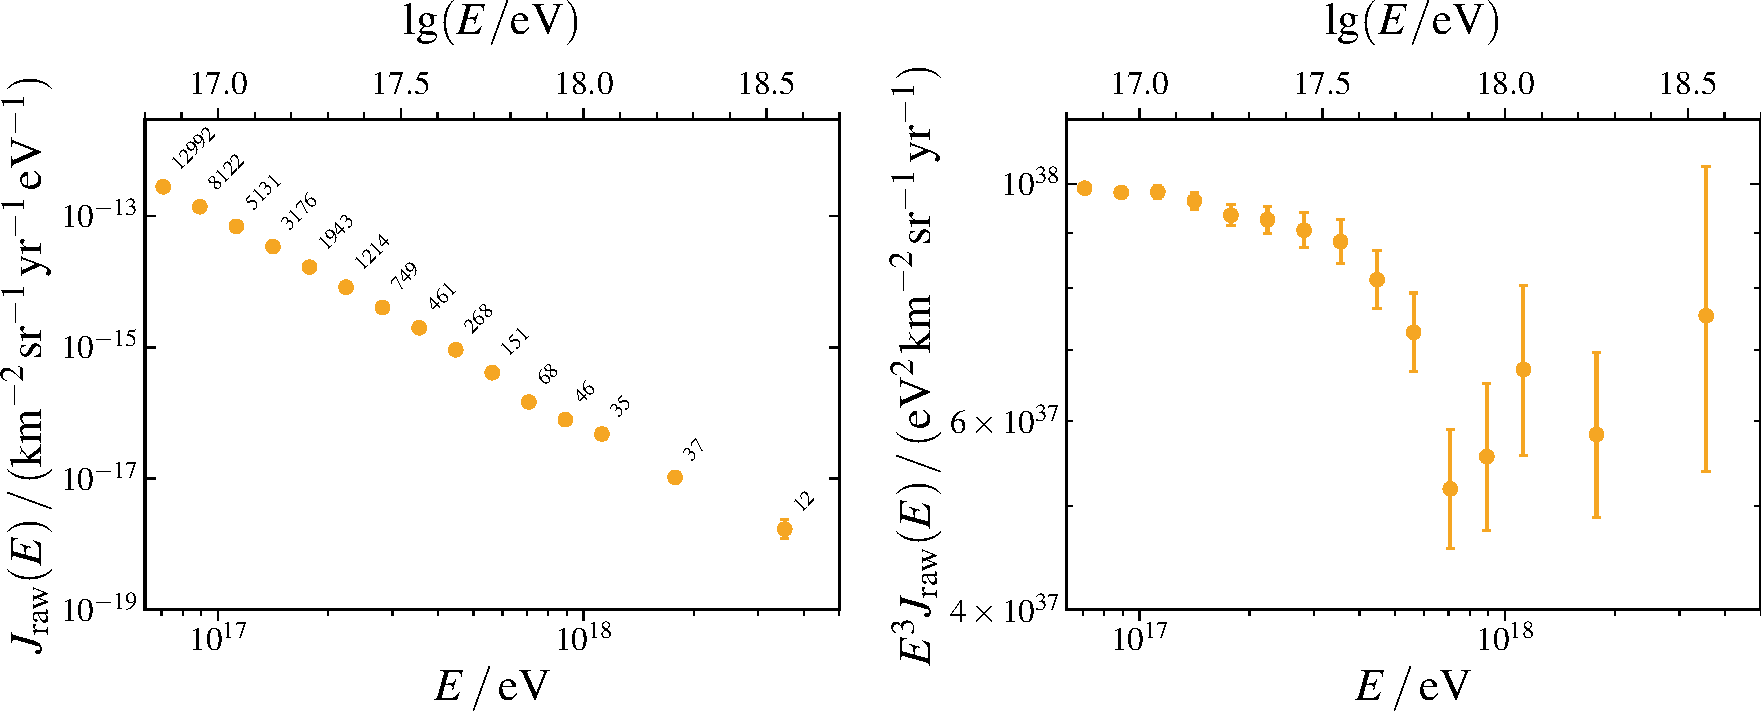
\includegraphics[width=\linewidth]{figures/chapter_spectrum/sd433_raw_spectrum.pdf}
    \caption{
        Raw cosmic-ray spectrum measured with the \sd{433}. The error bars represent the $68\%$ Poisson confidence intervals.
        Left: differential flux as a function of reconstructed energy; the numbers indicate the number of events in each bin.
        Right: the same flux multiplied by $E^3$ to highlight changes in spectral slope.}
    \label{fig:raw_spectrum}
\end{figure}

%%%%%%%%%%%%%%%%%%%%%%%%%%%%%%%%%%%%%%%%%%%%%%%%%%%%%%%%%%%%%%%%%%%%%%%%%%%
\section{Forward folding}
\label{forward_folding}
%%%%%%%%%%%%%%%%%%%%%%%%%%%%%%%%%%%%%%%%%%%%%%%%%%%%%%%%%%%%%%%%%%%%%%%%%%%
The detector response can be accounted for using either unfolding or forward folding.
In unfolding, the measured reconstructed-energy distribution is corrected to estimate the underlying true-energy distribution.
This inverse problem often requires regularization because a direct inversion of the detector response can amplify statistical fluctuations~\cite{Cowan:1998:StatisticalDataAnalysis,Lista:2023:StatisticalMethods}.
In forward folding, a model of the true-energy spectrum is convolved with the detector response, and the resulting reconstructed-energy distribution is compared directly with the measured counts.
The latter approach is used here because it avoids a direct inversion and incorporates the finite energy resolution, energy bias, and detection efficiency into the likelihood.

The finite energy resolution spreads events around their mean reconstructed energy, while the energy bias shifts this mean relative to the true energy.
Consequently, events from a given true-energy bin can be assigned to neighboring reconstructed-energy bins, while the detection efficiency determines the fraction of events that are detected.
These effects are represented by a migration matrix,


\begin{align}
R_{ij}
&=
\frac{
    \displaystyle
    \int_{\Delta E_i^{\mathrm{rec}}} \mathrm{d}E_{\mathrm{rec}}
    \int_{\Delta E_j^{\mathrm{true}}} \mathrm{d}E_{\mathrm{true}}\,
    J(E_{\mathrm{true}})\,\epsilon(E_{\mathrm{true}})\,
    \kappa(E_{\mathrm{rec}}\mid E_{\mathrm{true}})
}{
    \displaystyle
    \int_{\Delta E_j^{\mathrm{true}}}
    \mathrm{d}E_{\mathrm{true}}\,J(E_{\mathrm{true}})
},
\label{eq:migration_matrix}
\end{align}

The detector response $\kappa(E_{\mathrm{rec}}\mid E_{\mathrm{true}})$ is the conditional probability density for reconstructing $E_{\mathrm{rec}}$ given $E_{\mathrm{true}}$.
The detector efficiency $\epsilon(E_{\mathrm{true}})$, determined in \cref{sec:efficiency}, gives the probability that an event is detected.
Above full efficiency, elements $R_{ij}$ represent the probability that an event with true energy in bin $j$ is reconstructed in bin $i$.
However, at lower energies, where the efficiency is smaller than unity, the matrix also accounts for the probability that an event is detected, thereby allowing contributions from true energies below the full-efficiency threshold to be included.

The response function is modeled as a Gaussian distribution,
\begin{align}
    \kappa(E_{\mathrm{rec}}\mid E_{\mathrm{true}})
    &=
    \frac{1}{\sqrt{2\pi}\,\sigma(E_{\mathrm{true}})}
    \exp\left[
        -\frac{
            \left(
                E_{\mathrm{rec}}-E_{\mathrm{true}}
                \left[1+b(E_{\mathrm{true}})\right]
            \right)^2
        }{
            2\sigma^2(E_{\mathrm{true}})
        }
    \right],
    \label{eq:resolution_function}
\end{align}
where $\sigma(E_{\mathrm{true}})$ is the energy resolution and $b(E_{\mathrm{true}})$ is the relative energy bias, as determined from the simulations in \cref{sec:res_and_bias}.

At high energies, the relative resolution $\sigma(E_{\mathrm{true}})/E_{\mathrm{true}}$ approaches a constant value because shower-to-shower fluctuations dominate.
Consequently, the migration pattern retains approximately the same width and shape in logarithmic energy and is translated along the diagonal as $E_{\mathrm{true}}$ increases.
For a spectrum model parameterized by $\mathbf{s}$, the expected number of events in true-energy bin $j$ is
\begin{align}
    \mu_j(\mathbf{s})
    =
    \int_{\Delta E_j^{\mathrm{true}}}
    \mathrm{d}E_{\mathrm{true}}\,
    J(E_{\mathrm{true}}\mid\mathbf{s})
    \,\exposuresym(E_{\mathrm{true}}),
    \label{eq:expected_true_counts}
\end{align}
where $\exposuresym(E_{\mathrm{true}})$ denotes the exposure.
The spectrum is reported only above the full-efficiency threshold in order to minimize its dependence on the efficiency model.
After folding with the migration matrix, the expected number of events in the reconstructed-energy bin $i$ is
\begin{align}
    \nu_i(\mathbf{s})
    =
    \sum_j R_{ij}\,\mu_j(\mathbf{s}).
    \label{eq:expected_reconstructed_counts}
\end{align}

The spectrum parameters are determined by comparing the expected number of events $\nu_i$ with the observed number of events $n_i$ in each reconstructed-energy bin using a binned Poisson likelihood.
For this purpose, the Poisson deviance,
\begin{align}
    D(\mathbf{s})
    =
    2\sum_i
    \left[
        \nu_i(\mathbf{s})-n_i
        +
        n_i\ln\left(
            \frac{n_i}{\nu_i(\mathbf{s})}
        \right)
    \right],
    \label{eq:poisson_deviance}
\end{align}
is minimized with respect to $\mathbf{s}$.
It should be noted that the migration matrix in \cref{eq:migration_matrix} explicitly depends on the spectrum model $J(E_{\mathrm{true}}\mid\mathbf{s})$.
Consequently, changes in the spectrum parameters $\mathbf{s}$ during the fit iterations require the matrix to be recalculated.
To avoid this expensive calculation, an approximate migration matrix is used, following the approach described in Appendix~C of \cite{PierreAuger:2020:Spectrum}.

If the true-energy bins are sufficiently narrow, the efficiency and response function can be approximated as constant within each bin and can be taken outside the true-energy integral.
The remaining integral of $J(E_{\mathrm{true}}\mid\mathbf{s})$ in the numerator becomes identical to that in the denominator of \cref{eq:migration_matrix}, and the dependence on $J(E_{\mathrm{true}}\mid\mathbf{s})$ cancels out.
This yields the approximate migration matrix,
\begin{align}
    R_{ij}^{\mathrm{approx}}
    =
    \epsilon(E_j^{\mathrm{true}})
    \int_{\Delta E_i^{\mathrm{rec}}}
    \mathrm{d}E_{\mathrm{rec}}\,
    \kappa(E_{\mathrm{rec}}\mid E_j^{\mathrm{true}}).
    \label{eq:matrix_approx}
\end{align}

For the numerical calculation, the true-energy bin width is chosen as $\Delta\lg(E_j^{\mathrm{true}}/\mathrm{eV})=0.01$, while the reconstructed-energy bin width is $\Delta\lg(E_i^{\mathrm{rec}}/\mathrm{eV})=0.1$.
The approximate migration matrix for the \sd{433} is shown in \cref{fig:migration_matrix}, together with the full-efficiency threshold (red) and the identity (white).
The horizontal axis represents the true energy, while the vertical axis represents the reconstructed energy.
To avoid border effects, the migration matrix is calculated from $10^{16}$ to $10^{19}\,\mathrm{eV}$, thereby extending below the full-efficiency threshold and above the maximum reconstructed energy in the dataset.

\begin{figure}
    \centering
    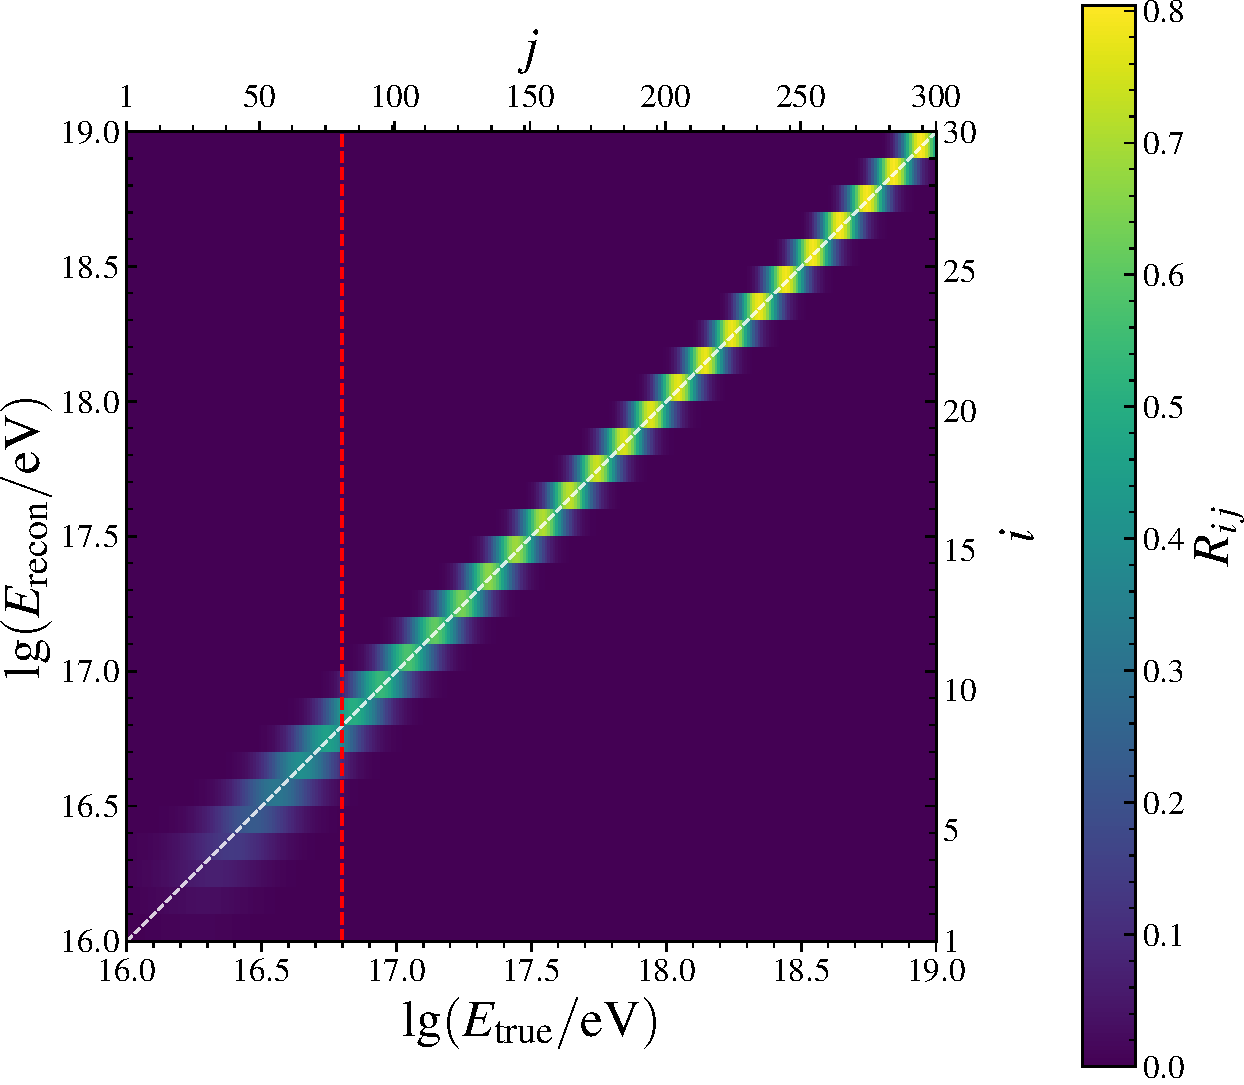
\includegraphics[width=0.75\linewidth]{figures/chapter_spectrum/sd433_migration_matrix.pdf}
    \caption{
        Approximate migration matrix for the \sd{433}.
        The horizontal axis represents true energy and the vertical axis reconstructed energy.
        The red dashed line indicates the full-efficiency threshold in true energy, and the white dashed line indicates
        $E_{\mathrm{rec}}=E_{\mathrm{true}}$.
    }
    \label{fig:migration_matrix}
\end{figure}

Although the spectrum is evaluated only for reconstructed energies above the full-efficiency threshold, upward energy fluctuations can reconstruct events with true energies below the threshold within the analysis range.
For the energy resolution and binning used here, the first two true-energy bins below the threshold contribute to the lowest reconstructed-energy bins of the spectrum.
Their reduced detection probability is incorporated through the efficiency factor $\epsilon(E_{\mathrm{true}})$ in the migration matrix, while contributions from lower true energies are negligible.

The next step is to evaluate the usefulness of this approximate matrix by comparing the expected number of events in reconstructed-energy bins predicted with the exact and approximate matrices, for the same underlying true-energy distribution.
To assess the accuracy of the approximation, a power-law spectrum,
\begin{align}
    J(E_{\mathrm{true}})=J_0E_{\mathrm{true}}^\gamma,
\end{align}
is used, with spectral index $\gamma=-3$.
The expected event numbers $\nu_i^{\mathrm{approx}}$ and $\nu_i^{\mathrm{exact}}$ are calculated using $R_{ij}^{\mathrm{approx}}$ and $R_{ij}^{\mathrm{exact}}$, respectively.
The relative difference,
\begin{align}
    \delta\nu_i
    =
    \frac{
        \nu_i^{\mathrm{approx}}
        -
        \nu_i^{\mathrm{exact}}
    }{
        \nu_i^{\mathrm{exact}}
    },
\end{align}
is shown in \cref{fig:nu_ratio}.

\begin{figure}
    \centering
    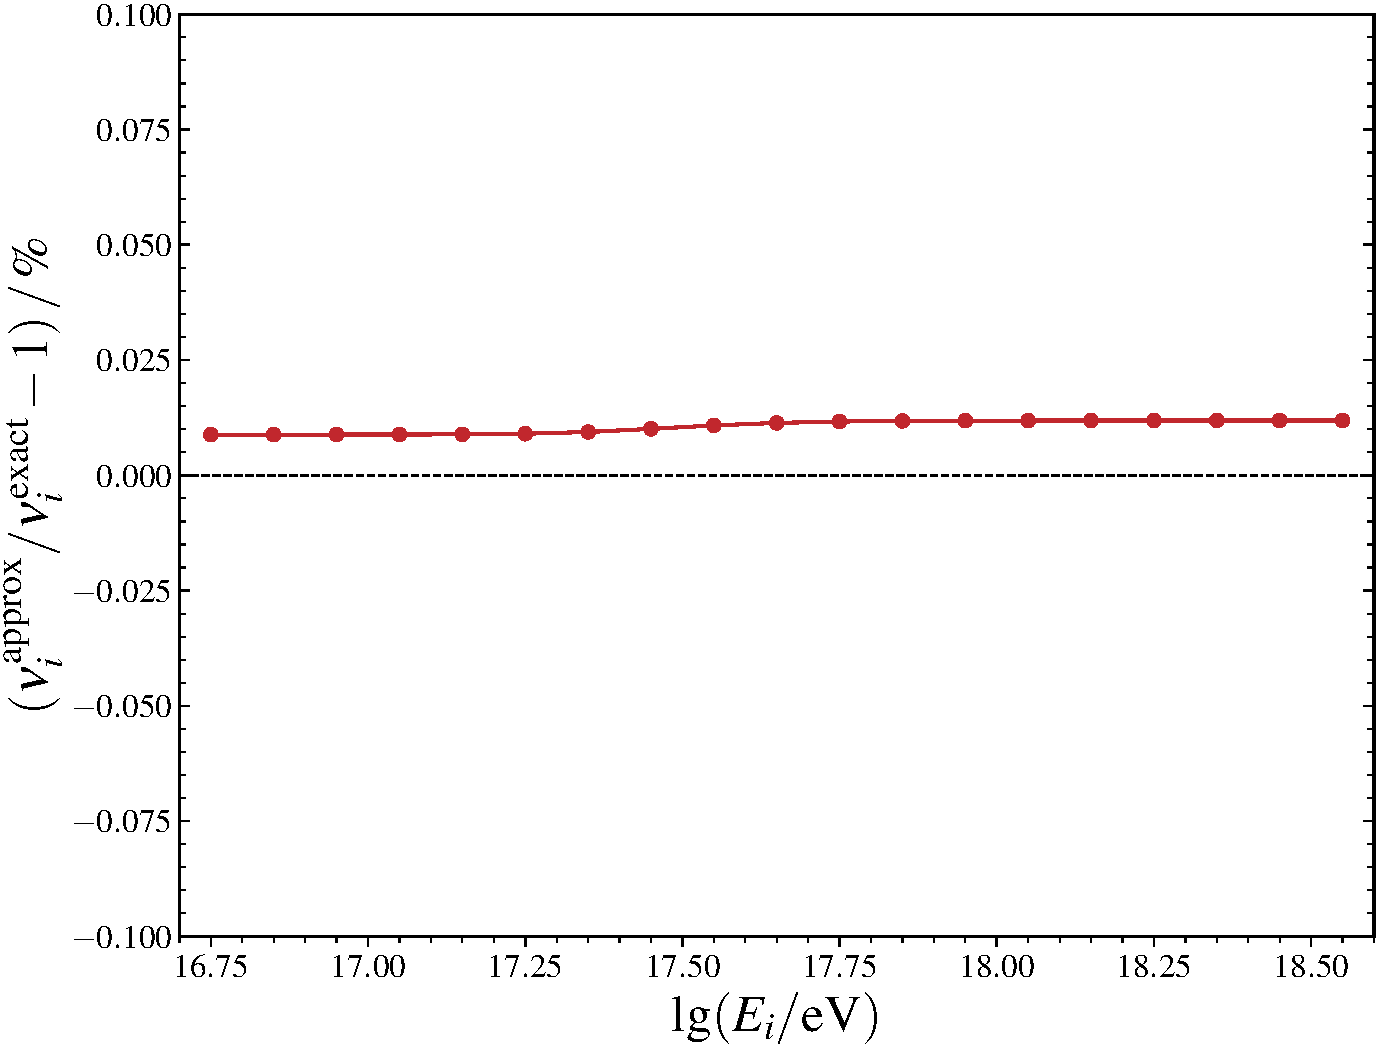
\includegraphics[width=0.75\linewidth]{figures/chapter_spectrum/nu_ratio.pdf}
    \caption{
        Relative difference between the expected event numbers obtained using the approximate and exact migration matrices for a power-law spectrum with $\gamma=-3$.
    }
    \label{fig:nu_ratio}
\end{figure}

The difference remains below $0.02\%$ over the full energy range, indicating that the effect of the approximation is negligible for the chosen binning.
The approximate matrix is therefore used in the forward-folding fit.
It avoids recalculating the exact, spectrum-dependent matrix at every iteration and does not require an a priori spectrum close to the final solution for numerical convergence.

The best-fit spectrum parameters $\hat{\mathbf{s}}$ are determined using the procedure described above.
Subsequently, the ratio,
\begin{align}
    c_i
    =
    \frac{
        \mu_i(\hat{\mathbf{s}})
    }{
        \nu_i(\hat{\mathbf{s}})
    },
    \label{eq:correction_factor}
\end{align}
is calculated in each bin.

The corrections are less than 7\% over the full energy range of the \sd{433} spectrum, as shown in \cref{fig:correction_factors}.
These correction factors are more relevant near the full-efficiency threshold, where the energy resolution has the greatest impact on the migration of events.
At high energies, they become approximately constant because relative shower-to-shower fluctuations, assumed to be energy-independent, dominate.

\begin{figure}
    \centering
    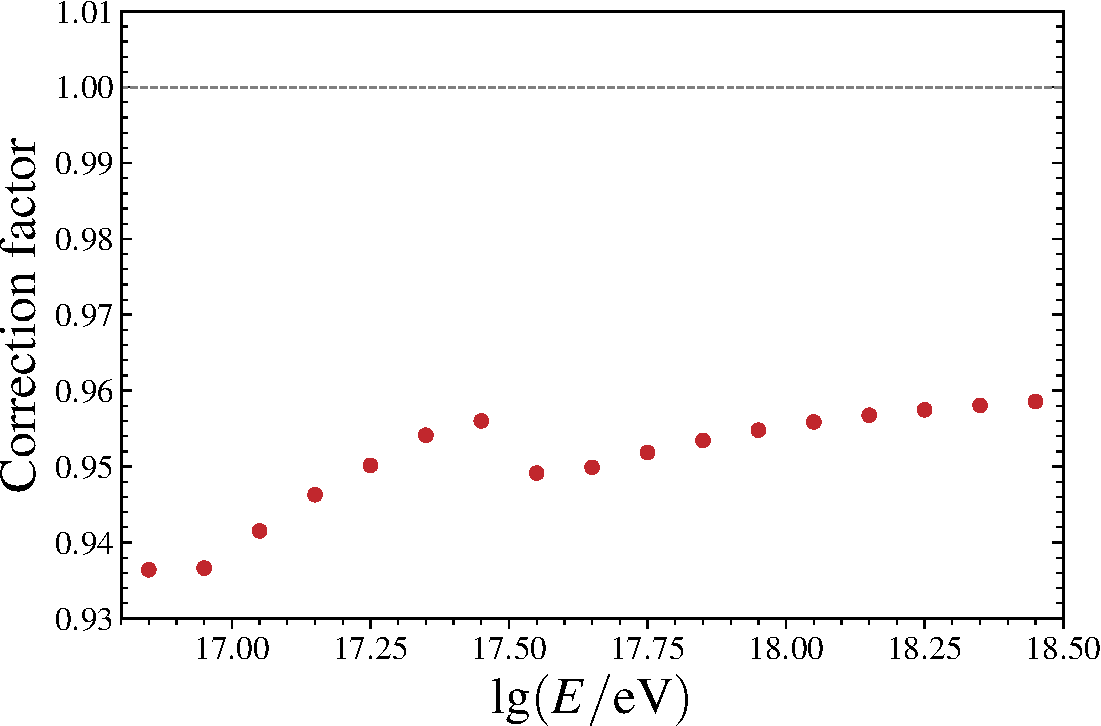
\includegraphics[width=0.75\linewidth]{figures/chapter_spectrum/sd433_nominal_correction_factors.pdf}
    \caption{
        Correction factors obtained from the forward-folding fit to the measured \sd{433} dataset.
    }
    \label{fig:correction_factors}
\end{figure}

%%%%%%%%%%%%%%%%%%%%%%%%%%%%%%%%%%%%%%%%%%%%%%%%%%%%%%%%%%%%%%%%%%%%%%%%%%%
\section{The \sd{433} Unfolded spectrum}
\label{sec:unfolded_spectrum}
%%%%%%%%%%%%%%%%%%%%%%%%%%%%%%%%%%%%%%%%%%%%%%%%%%%%%%%%%%%%%%%%%%%%%%%%%%%


The correction factors are then used to estimate the unfolded flux $J_i$ from the measured flux,
\begin{align}
    J_i
    =
    c_i J_i^{\mathrm{raw}}.
\end{align}

The \sd{433} spectrum is fitted between $\lg(E/\mathrm{eV})=16.8$ and $18.5$.
The lower limit is determined by the full-efficiency threshold, and the upper limit is chosen below the ankle so that the second knee can be determined without requiring an additional spectral feature.

To test for the presence of a knee-like structure in the spectrum, the data are first fitted with a simple power law,
\begin{align}
    J(E)
    =
    J_0
    \left(
        \frac{E}{10^{17}\,\mathrm{eV}}
    \right)^{-\gamma},
\end{align}
where the normalization $J_0$ and spectral index $\gamma$ are free parameters.
The resulting fit, shown in \cref{app:chap_spectrum}, yields a Poisson deviance of
$D/\mathrm{dof}=\SDFourThreeThreePowerLawDeviance/\SDFourThreeThreePowerLawDof$,
corresponding to a $p$-value of $\SDFourThreeThreePowerLawPValue$.
The simple-power-law hypothesis is therefore rejected, providing strong evidence for a change in the spectral slope within the measured energy range.
Consequently, a broken power law with a soft transition is used to fit the spectrum,
\begin{align}
    J(E)=J_0\left(
    \frac{E}{10^{17}\,\mathrm{eV}}
    \right)^{-\gamma_0}
    \left[
    1+\left(
    \frac{E}{E_{01}}
    \right)^{\frac{1}{\omega_{01}}}
    \right]^{(\gamma_0-\gamma_1)\omega_{01}},
    \label{eq:bplwst}
\end{align}
where $J_0$ is the normalization factor.
The second knee is characterized by its energy $E_{01}$, the spectral indices $\gamma_0$ and $\gamma_1$ before and after the feature, respectively, and $\omega_{01}$, which governs the width of the transition~\cite{PierreAuger:2021:InfillSpectrum}.

The spectrum is first fitted with all five parameters left free.
The fit converges and yields a Poisson deviance of
$D/\mathrm{dof}=12.3/12$, corresponding to a $p$-value of $0.42$.
The best-fit parameters are listed in \cref{table:sd433_fits_omega}.
Although the second-knee energy and spectral indices are well constrained, the transition width is found to be $\omega_{01}=0.09\pm0.27$.
The uncertainty is considerably larger than the best-fit value, and the corresponding symmetric interval includes unphysical negative values, indicating that the \sd{433} data cannot constrain the width of the transition.


\begin{table}
    \centering
    \caption{
        Spectral parameters and fit quality for the \sd{433} spectrum obtained with $\omega_{01}$ left free and with $\omega_{01}$ fixed to $0.05$. Quoted uncertainties are statistical.
    }
    \label{table:sd433_fits_omega}
    \begin{tabular}{lcc}
        \hline
        Parameter
        & $\omega_{01}$ free
        & $\omega_{01}=0.05$ (fixed) \\
        \hline
        $J_0/
        \left(
        10^{-13}\,
        \mathrm{km^{-2}\,yr^{-1}\,sr^{-1}\,eV^{-1}}
        \right)$
        & $0.913\pm0.007$
        & $0.913\pm0.005$ \\
        $\lg(E_{01}/\mathrm{eV})$
        & $17.44\pm0.09$
        & $17.44\pm0.08$ \\
        $\gamma_0$
        & $3.03\pm0.03$
        & $3.04\pm0.02$ \\
        $\gamma_1$
        & $3.34\pm0.08$
        & $3.34\pm0.08$ \\
        $\omega_{01}$
        & $0.09\pm0.27$
        & $0.05$ (fixed) \\
        $D/\mathrm{dof}$
        & $12.3/12$
        & $12.3/13$ \\
        $p$-value
        & $0.42$
        & $0.50$ \\
        \hline
    \end{tabular}
\end{table}

Therefore, we perform a second fit fixing $\omega_{01}=0.05$, the same value adopted by the Pierre Auger Observatory for spectral features whose transition widths could not be constrained~\cite{PierreAuger:2020:Spectrum}.
This fit also provides a good description of the data.
Leaving the transition width free keeps the deviance stable, while introducing an additional fit parameter.
The reconstructed second-knee energy and spectral indices are compatible between the two fits within their uncertainties. Moreover, the inability to constrain $\omega_{01}$ does not significantly affect the determination of the other spectral parameters.
Consequently, the transition width is fixed in the \sd{433}-only spectrum measurement.
Although subdominant, the influence of $\omega_{01}$ on the measured spectrum is examined further in \cref{subsec:transition_systematic}, together with other sources of systematic uncertainty.

The resulting unfolded spectrum and the residuals with respect to the fitted model are shown in \cref{fig:sd433_unfolded_spectrum}.
\begin{figure}
    \centering
    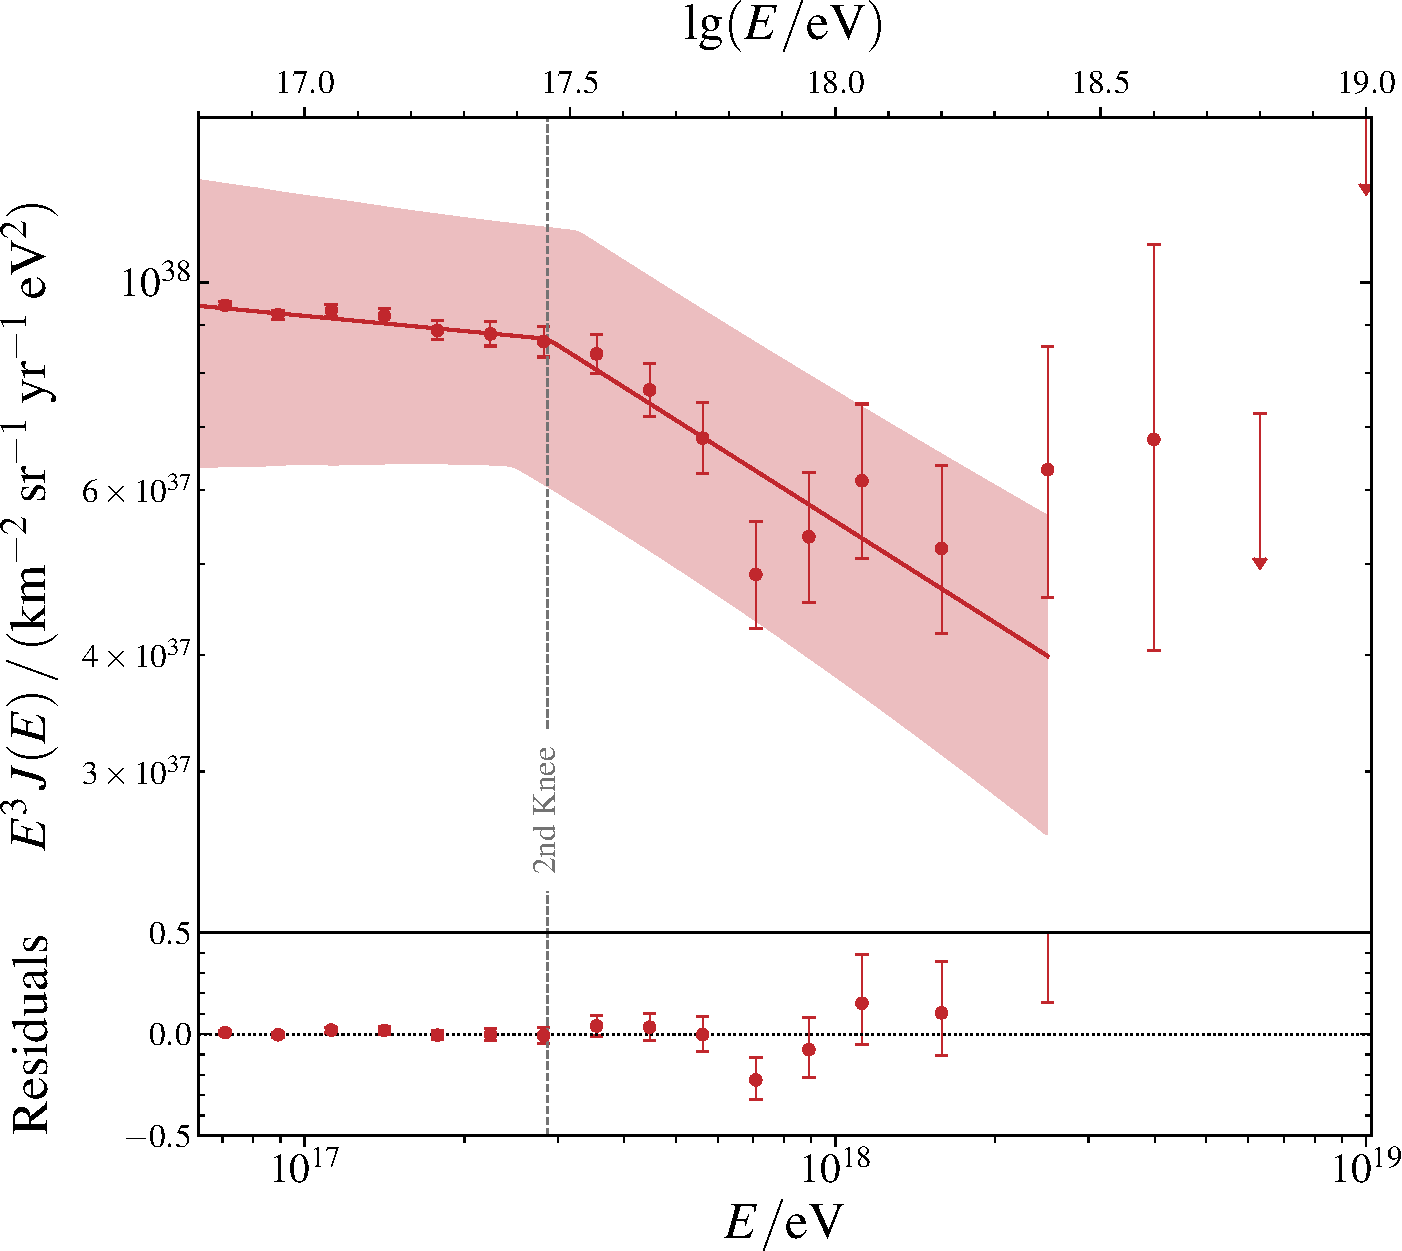
\includegraphics[width=0.8\linewidth]{figures/chapter_spectrum/sd433_unfolded_spectrum_with_residuals.pdf}
    \caption{Unfolded cosmic-ray spectrum measured with the \sd{433} and the best-fit broken power law with a smooth transition. The lower panel shows the residuals with respect to the fitted model.}
    \label{fig:sd433_unfolded_spectrum}
\end{figure}

To assess the stability of the spectral parameters, the fit was repeated by progressively increasing the minimum fit energy from $\lg(E_{\min}/\mathrm{eV})=16.8$ to $17.2$.
The results are shown in \cref{fig:sd433_fit_min_stability}.
The reconstructed second-knee energy and spectral indices remain compatible within statistical uncertainties over the full range.
As the minimum energy increases, the number of events and the lever arm below the second knee decrease.
Consequently, the uncertainty in $\gamma_0$ increases; however, the fitted value remains compatible with the nominal result at $\lg(E_{\min}/\mathrm{eV})=16.8$.

\begin{figure}
    \centering
    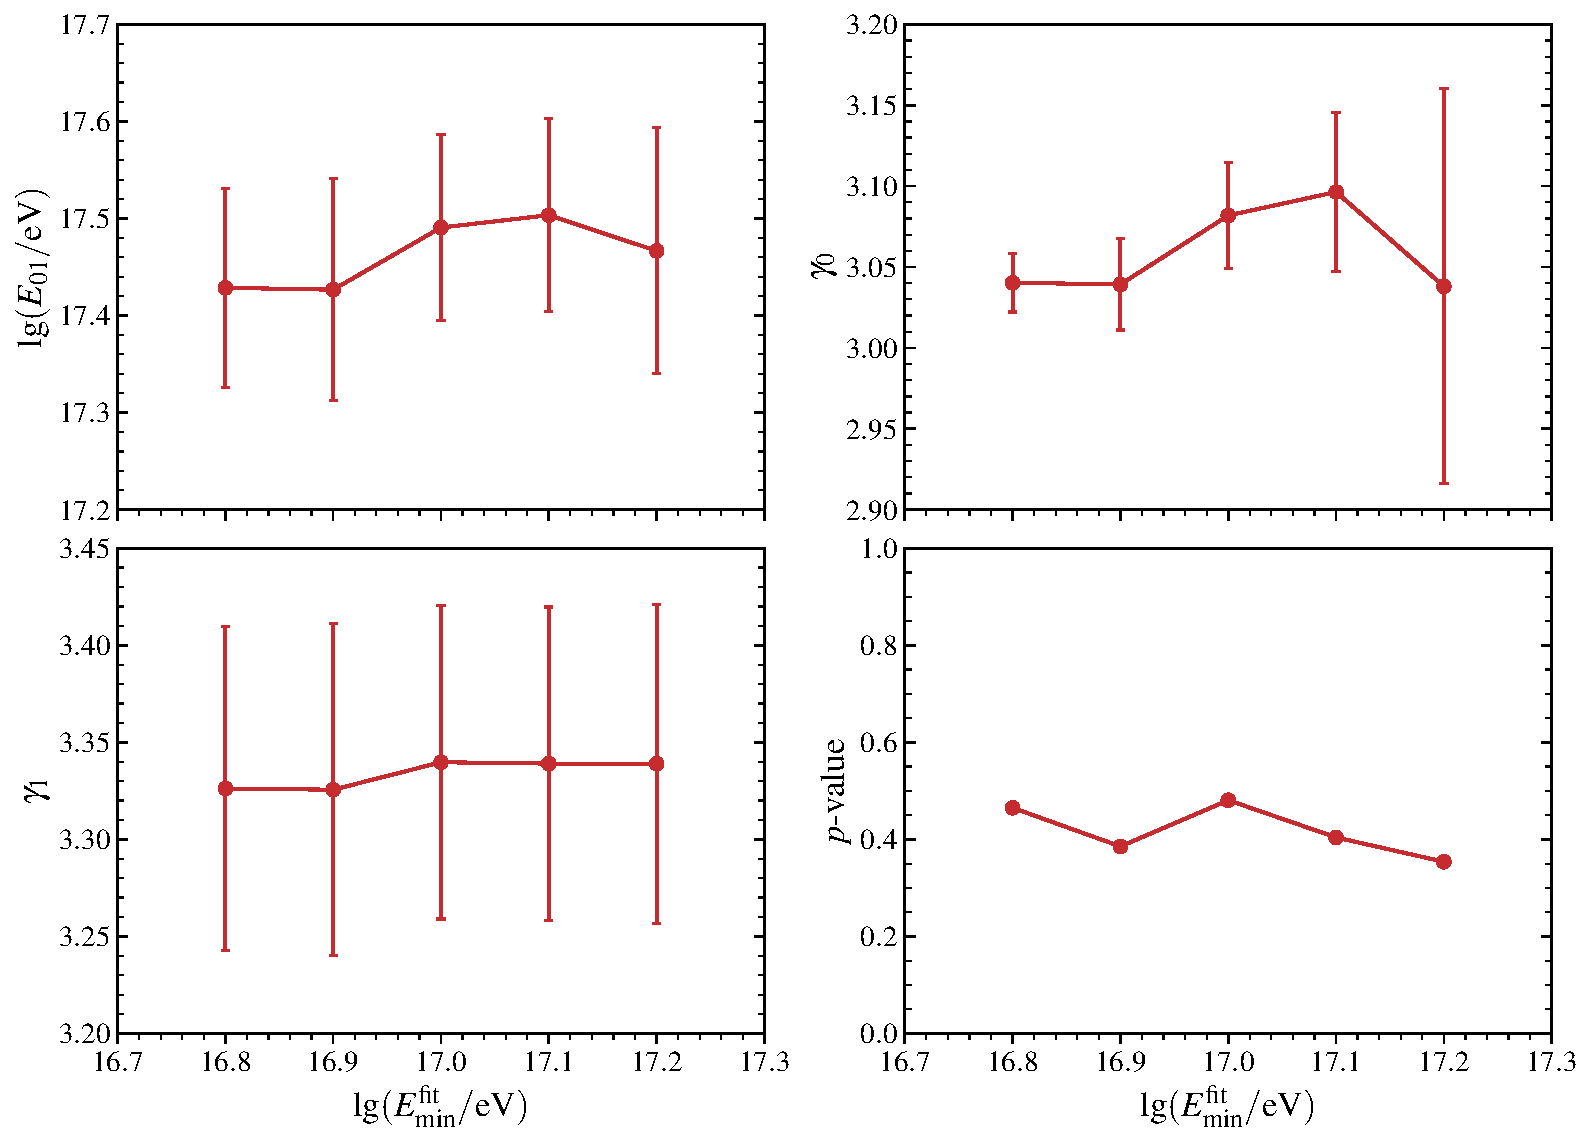
\includegraphics[width=\linewidth]
    {figures/chapter_spectrum/sd433_fit_min_stability_2x2.pdf}
    \caption{
        Dependence of the fitted second-knee parameters and the goodness-of-fit $p$-value on the minimum energy included in the fit.
        The error bars represent the statistical uncertainties of the fitted parameters.
        The $p$-value is calculated from the Poisson deviance using the corresponding number of degrees of freedom.
    }
    \label{fig:sd433_fit_min_stability}
\end{figure}

%%%%%%%%%%%%%%%%%%%%%%%%%%%%%%%%%%%%%%%%%%%%%%%%%%%%%%%%%%%%%%%%%%%%%%%%%%%
\section{Spectrum systematics}
\label{sec:systematics}
%%%%%%%%%%%%%%%%%%%%%%%%%%%%%%%%%%%%%%%%%%%%%%%%%%%%%%%%%%%%%%%%%%%%%%%%%%%

The systematic uncertainties affecting the \sd{433} spectrum arise from the exposure, the energy scale, the detector response, and the assumed transition width.
The dominant contribution is the approximately $14\%$ energy-scale uncertainty inherited from the calibration of the \sd{750} with the FD.

The exposure uncertainty is approximately $3\%$ and is energy-independent, since the exposure is calculated geometrically from the number of active hexagons~\cite{PierreAuger:2010:TriggerAperture}.
The uncertainties associated with the detector response include the energy resolution and the composition dependence of the bias and efficiency.
The uncertainties in the calibration parameters determined in \cref{chapter:reconstruction} are also included.

These sources are treated as uncorrelated, and their effects on both the flux and the fitted spectral parameters are evaluated using the forward-folding procedure described in the previous section.
Their contributions are combined in quadrature to determine the total systematic uncertainty of the measurement.
The influence of the assumed value of $\omega_{01}$ on the determination of the second knee is assessed separately using the measured data and toy Monte Carlo simulations.

\subsection{FD energy systematic}

The calibration of the \gls{sd} with the \gls{fd} transfers the FD energy-scale systematic uncertainty to the \sd{433} spectrum.
The individual contributions to this uncertainty are described in detail in \cite{PierreAuger:2015:Observatory} and are summarized in \cref{table:energy_scale_systematics}.
The dominant contributions are the absolute calibration of the \gls{fd} and the reconstruction of the longitudinal shower profile.

\begin{table}
    \centering
    \caption{Contributions to the systematic uncertainty in the \gls{fd} energy scale. The ranges indicate the energy dependence of the corresponding contributions. The total uncertainty amounts to 14\,\%.}
    \label{table:energy_scale_systematics}
    \begin{tabular}{lr}
        \hline
        Fluorescence yield
            & 3.6\,\% \\
        Atmosphere
            & 3.4--6.2\,\% \\
        FD calibration
            & 9.9\,\% \\
        FD profile reconstruction
            & 5.6--6.5\,\% \\
        Invisible energy
            & 3--1.5\,\% \\
        Statistical uncertainty of the SD calibration fit
            & 0.7--1.8\,\% \\
        Stability of the energy scale
            & 5\,\% \\
        \hline
        \textbf{Total}
            & \textbf{14\,\%} \\
        \hline
    \end{tabular}
\end{table}

Some contributions exhibit a mild energy dependence, while the total uncertainty is approximately energy independent and amounts to $14\%$.

The effect of the energy-scale uncertainty on the spectrum is evaluated analytically and cross-checked numerically by coherently shifting the reconstructed energies of the measured events.

For a relative shift $\delta$ in the energy scale, the shifted energy is $E'=(1+\delta)E$, with $\delta=\pm0.14$.
The corresponding change in the flux follows from the transformation of a probability density,
\begin{align}
    J'(E')=J(E)\left|\frac{dE}{dE'}\right|,
    \label{eq:change_of_variables}
\end{align}
where $J(E)$ and $J'(E')$ are the differential fluxes on the original and shifted energy scales, respectively.
For a flux of general shape, \cref{eq:change_of_variables} can be expanded as,
\begin{align}
\frac{\Delta J(E)}{J(E)}
=
\frac{1}{1+\delta}
\frac{
J\left(\frac{E}{1+\delta}\right)
}{
J(E)
}
-1,
\label{eq:energy_systematic_bplwst}
\end{align}
The analytical estimate of the systematic uncertainty obtained from the fitted \sd{433} spectrum is shown in \cref{fig:energy_systematic}.

As a numerical cross-check, the reconstructed energy of every event is shifted by $\delta=\pm0.14$, and the complete forward-folding and unfolding procedures are repeated.
The migration matrix is kept unchanged because the energy-scale shift does not modify the assumed detector resolution, bias, or efficiency.
The corresponding unfolded spectra are shown in \cref{appendix_chapter_spectrum}.

The flux variations obtained with this procedure are also shown in \cref{fig:energy_systematic}.
The forward-folding and analytical results agree over most of the energy range.
The differences above the second knee arise from the limited statistics above the feature, which hinder a stable estimate of the systematics obtained by shifting event energies.
Therefore, the analytical method is better suited to provide a stable estimate of the systematic uncertainty over the full energy range.

\begin{figure}
    \centering
    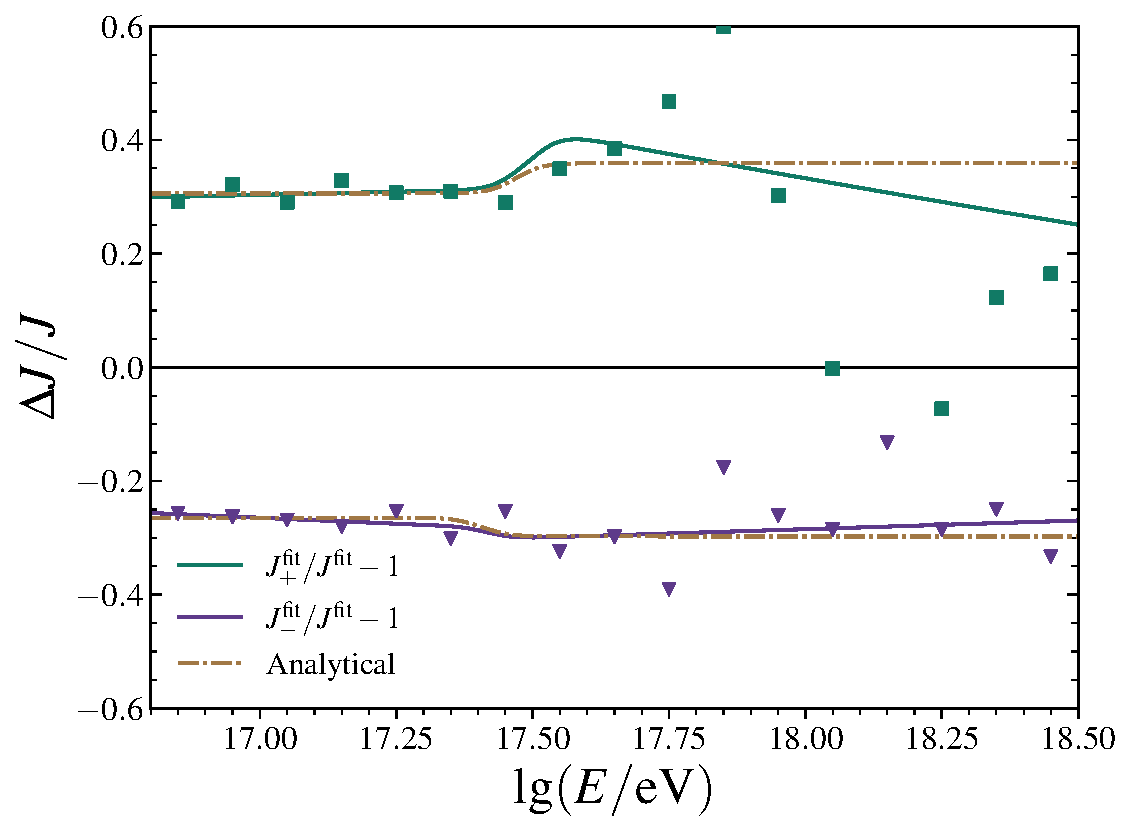
\includegraphics[width=0.8\linewidth]{figures/chapter_spectrum/delta_j_over_j.pdf}
    \caption{Relative change in the flux for coherent energy-scale shifts of $+14\%$ and $-14\%$. The points show the unfolded-flux variations, the solid curves show the results obtained by repeating the forward-folding fit, and the dash-dotted curves show the analytical estimate from \cref{eq:energy_systematic_bplwst}.}
    \label{fig:energy_systematic}
\end{figure}

The method of shifting event energies is applied to evaluate the systematic uncertainties of the spectral parameters, as shown in \cref{fig:energy_systematic_fit_parameters}.
\begin{figure}
    \centering
    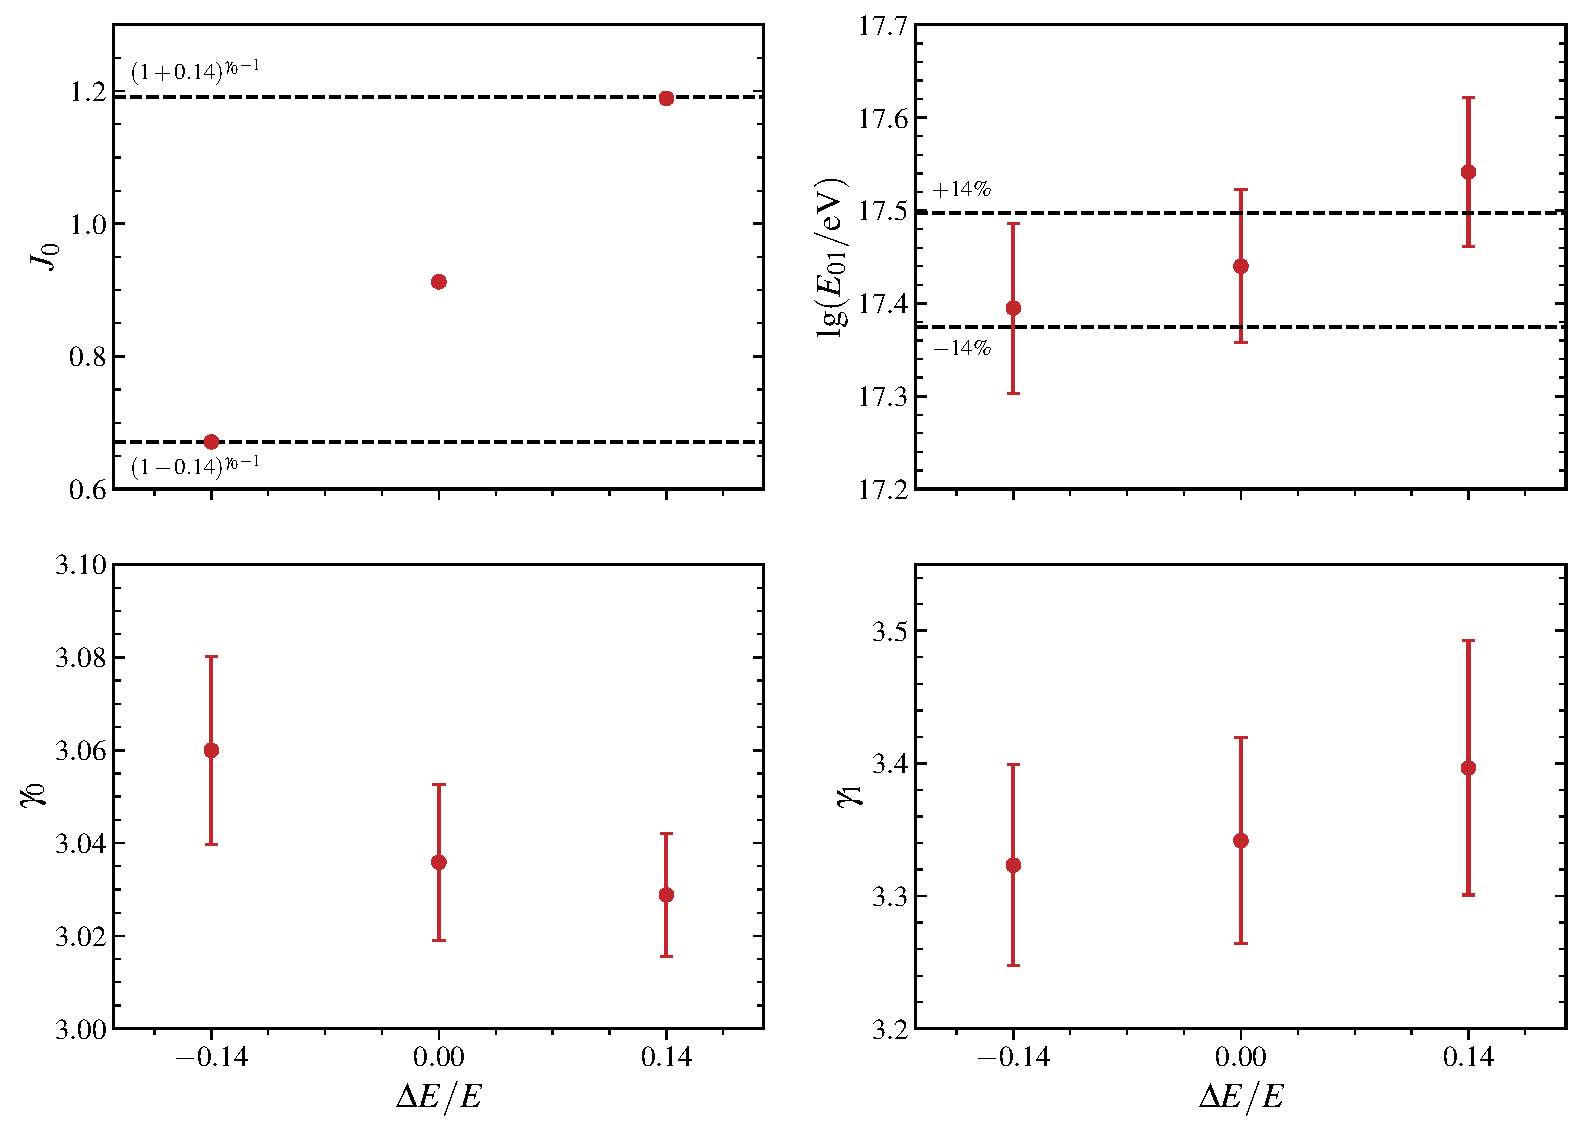
\includegraphics[width=\linewidth]{figures/chapter_spectrum/energy_systematic_fit_parameters.pdf}
    \caption{Fitted normalization $J_0$, second-knee energy $E_{01}$, and spectral indices $\gamma_0$ and $\gamma_1$ for the nominal energy scale and for coherent shifts of $+14\%$ and $-14\%$. The error bars show the statistical uncertainties of the fits. The dashed lines in the upper panels indicate the expectations obtained by directly propagating the energy-scale shift.}
    \label{fig:energy_systematic_fit_parameters}
\end{figure}

The fitted values of $\gamma_0$ and $\gamma_1$ remain consistent with the nominal values within their statistical uncertainties, as expected for a coherent shift of the energy scale.
For energy-scale shifts of $+14\%$ and $-14\%$, the fitted second-knee position changes by $+0.10$ and $-0.05$ in $\lg(E_{01}/\mathrm{eV})$, respectively.
The corresponding shifts expected from direct propagation of the energy scale are $+0.06$ and $-0.066$.
A conservative symmetric systematic uncertainty of $\Delta\lg(E_{01}/\mathrm{eV})=\pm0.10$ is therefore assigned, corresponding to the largest absolute variation obtained from the refits.


\subsection{Response function systematics}
\label{subsec:response_systematics}

The systematic uncertainties associated with the detector response are evaluated by varying independently the energy resolution, bias, and efficiency, within their respective uncertainties.
The contribution from the energy resolution is determined by varying the parameters of the resolution model defined in \cref{eq:resolution_sigma}, following the procedure in \cite{PierreAuger:2021:InfillSpectrum}.
The parameters $R_{\mathrm{sh}}$ and $R_0$ are shifted up and down by their respective $1\sigma$ uncertainties.
For each of these two variations, the migration matrix is recalculated while keeping the other components of the detector response unchanged, and the spectrum is fitted again.
The relative change in the fitted flux $\Delta J/J$ is calculated for each case and combined in quadrature to get the overall systematic uncertainty due to uncertainty in the energy resolution.
The contribution from the energy resolution is shown in the left panel of \cref{fig:sd433_systematic_budget}.
Its magnitude is largest near the full-efficiency threshold, where it reaches approximately $1.1\%$, and decreases with energy.
The resulting spectra and fitted parameters after shifting the resolution up and down are reported in \cref{appendix_chapter_spectrum}.

The dependence of the detector response on the assumed mass composition is estimated using the bias and efficiency parametrizations obtained in \cref{sec:res_and_bias} for pure proton and pure iron primaries.
The contributions of the energy bias and the trigger efficiency are evaluated separately, following the same procedure used for the uncertainty of the energy resolution.
%
The variation of the flux due to the assumed bias leaves the position of the second knee and the spectral indices essentially unchanged.
However, its contribution to $\Delta J/J$ reaches approximately $4.3\%$ near the full-efficiency threshold.
The composition dependence of the efficiency produces a smaller contribution to the flux uncertainty, with a maximum of approximately $1.5\%$, and shifts the position of the second knee downward by
$\Delta\lg(E_{01}/\mathrm{eV})=-0.03$.
%
The contributions from the energy bias and trigger efficiency are shown in the left panel of \cref{fig:sd433_systematic_budget}.

\subsection{Calibration systematic}
\label{subsec:calibration_systematic}

The energy assigned to each \sd{433} event is obtained from the calibration of its shower size with the \sd{750} energy estimator, described in \cref{sec:calibration}.
In addition to the uncertainty inherited from the FD energy scale, the finite precision of the calibration introduces an independent contribution to the spectrum uncertainty.
This contribution arises from the uncertainties in the normalization $A$ and slope $B$ of the calibration relation.
A variation of $A$ produces a uniform shift in energy, whereas a variation of $B$ produces an energy-dependent shift and therefore modifies the spectral indices.
%
The effect of the calibration slope can be understood analytically; for the calibration relation, a change from $B$ to $B'$, while keeping $A$ fixed, transforms the reconstructed energy according to,
\begin{align}
    E'
    =
    A
    \left(\frac{E}{A}\right)^{\frac{B'}{B}}.
    \label{eq:calibration_energy_transformation}
\end{align}
The corresponding transformation of the flux follows from the change of variables in \cref{eq:change_of_variables},
\begin{align}
    J'(E')
    =
    \frac{B}{B'}
    \frac{E}{E'}
    J(E).
    \label{eq:calibration_flux_transformation}
\end{align}
For a power-law spectrum, $J(E)\propto E^{-\gamma}$, the transformed spectrum is also a power law with spectral index,
\begin{align}
    \gamma'
    =
    1+(\gamma-1)\frac{B}{B'}.
    \label{eq:calibration_spectral_index}
\end{align}
This yields a change in the spectral index,
\begin{align}
    \Delta\gamma
    =
    (\gamma-1)
    \left(\frac{B}{B'}-1\right).
    \label{eq:calibration_spectral_index_change}
\end{align}


In the systematic evaluation, the calibration parameters are varied according to the systematic uncertainties determined in \cref{sec:calibration}.
The correlated variations used to define the systematic envelope are
$(A^+,B^-)=(125.7~\mathrm{PeV},0.909)$ and
$(A^-,B^+)=(113.3~\mathrm{PeV},0.983)$.
The nominal and varied calibration relations are shown in the left panel of \cref{fig:calibration_systematic}.
For each variation, the energy of every event is recalculated and the spectrum is fitted again.
The two resulting unfolded spectra are shown in the right panel of \cref{fig:calibration_systematic}.
\begin{figure}
    \centering
    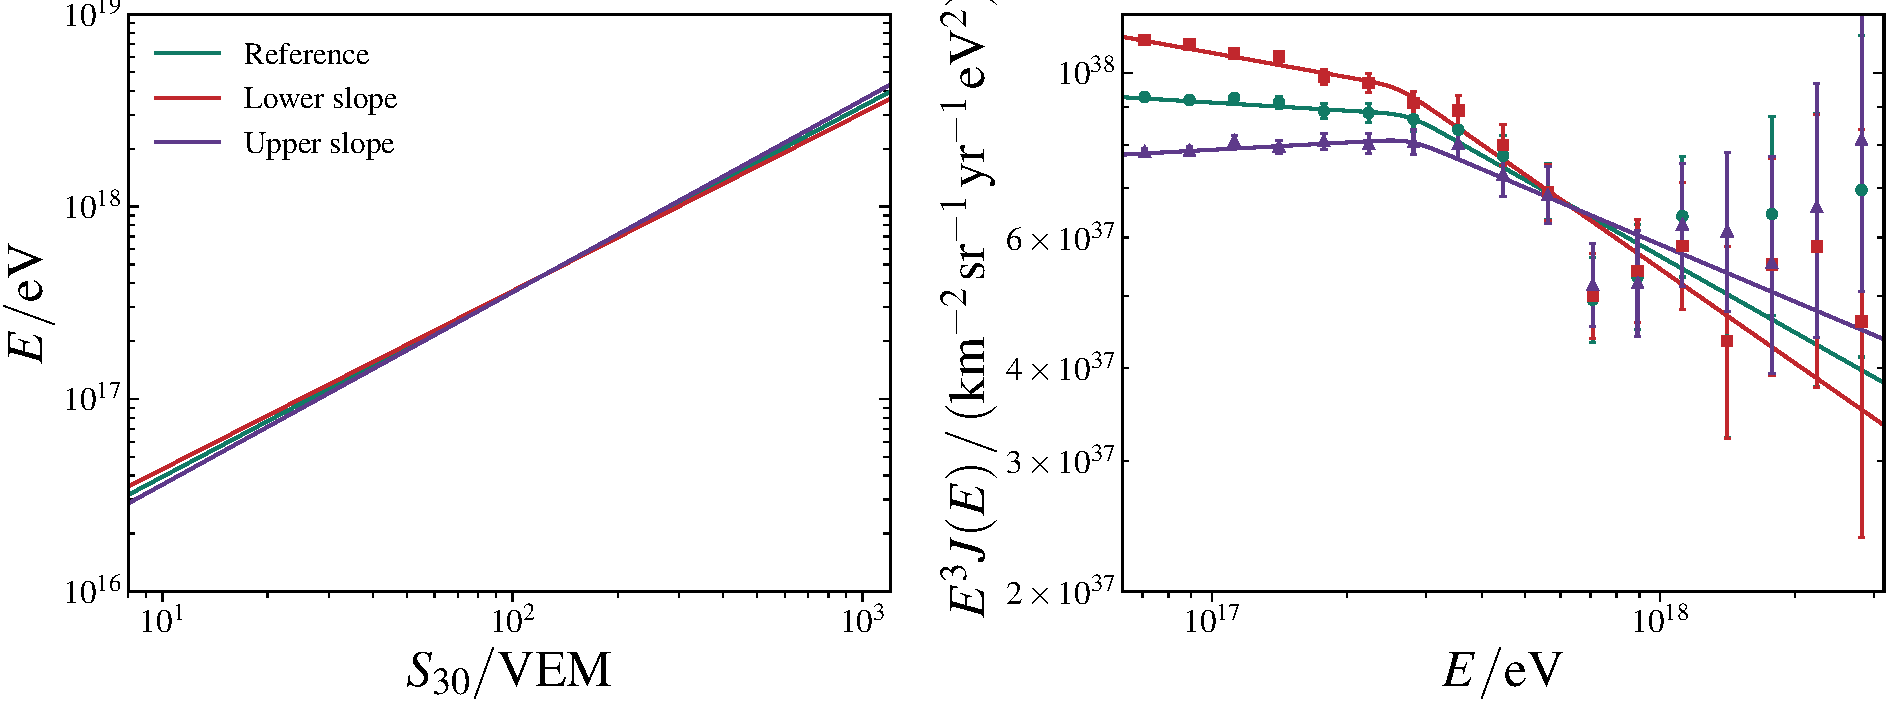
\includegraphics[width=\textwidth]{figures/chapter_spectrum/calibration_systematic.pdf}
    \caption{
        Effect of the calibration systematic on the reconstructed spectrum.
        The left panel shows the reference calibration relation together with the lower- and upper-slope variations.
        The right panel shows the corresponding unfolded spectra scaled by $E^3$ together with their respective fitted spectral functions.
    }
    \label{fig:calibration_systematic}
\end{figure}
Using the fitted values of the spectral indices, $\gamma_0=3.04$ and $\gamma_1=3.34$, $\Delta\gamma_0^{\mathrm{analytical}}=0.083$ and $\Delta\gamma_1^{\mathrm{analytical}}=0.095$ are predicted by \cref{eq:calibration_spectral_index_change}.
The corresponding changes obtained from the alternative method of shifting the event energies are
$\Delta\gamma_0^{\mathrm{fit}}=0.073$ and
$\Delta\gamma_1^{\mathrm{fit}}=0.081$.
The systematic uncertainties estimated with both methods agree with each other.
Since the analytical estimates are slightly larger, they are adopted as conservative systematic uncertainties.
A similar procedure is applied to estimate the contribution of the calibration uncertainty to the second-knee position, yielding $\Delta\lg(E_{01}/\mathrm{eV})=0.024$.

The contribution of the calibration to the flux uncertainty is shown in the right panel of \cref{fig:systematic_budget}.
It is the second-largest contribution after the energy-scale uncertainty and
its magnitude is largest at the boundaries of the energy range, reaching
$19\%$ at $\lg(E/\mathrm{eV})=16.8$ and
$13\%$ at $\lg(E/\mathrm{eV})=18.5$.
The right panel of \cref{fig:systematic_budget} also shows the contributions from the exposure and unfolding assumptions, together with the total uncertainty obtained by combining all contributions in quadrature.
\begin{figure}
    \centering
    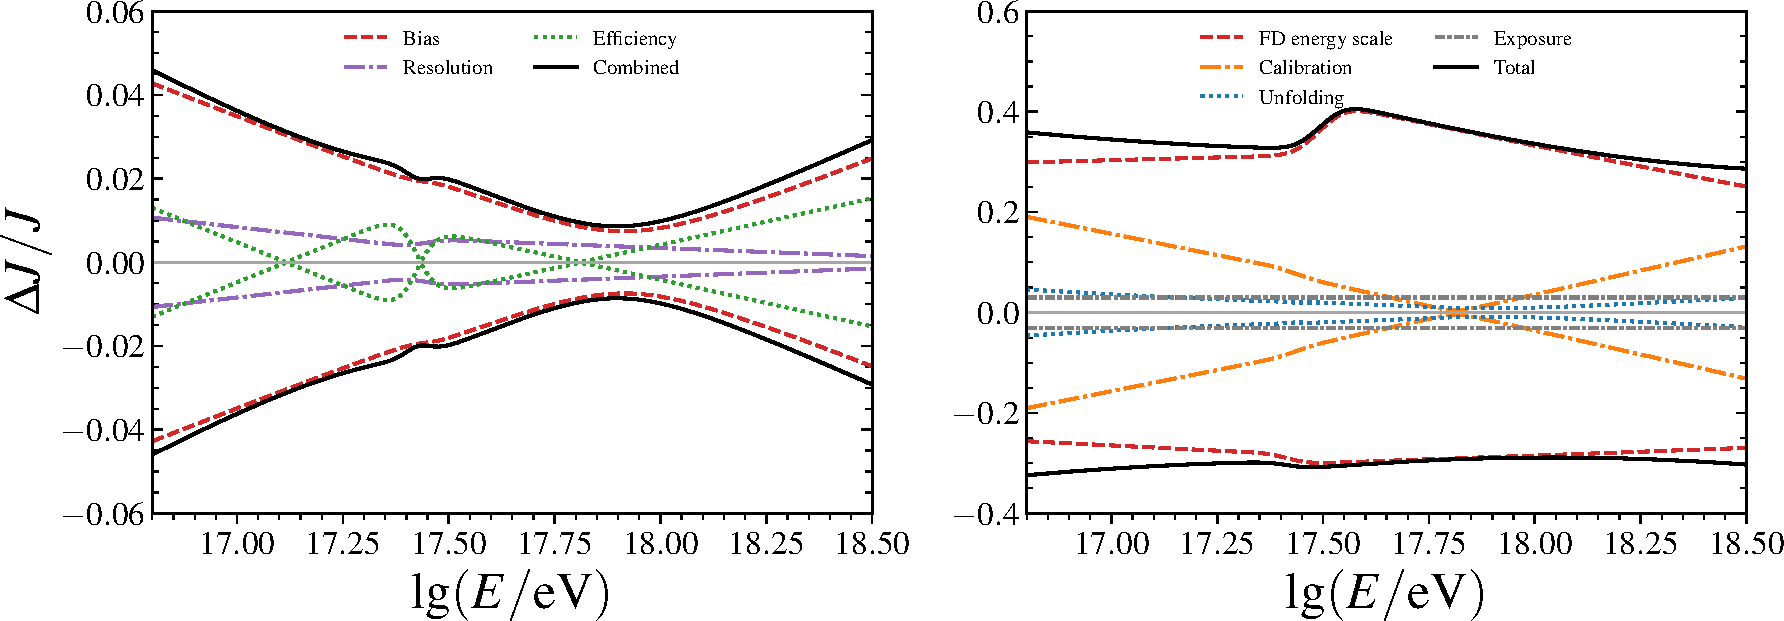
\includegraphics[width=\linewidth]{figures/chapter_spectrum/sd433_systematic_budget.pdf}
    \caption{Relative systematic uncertainty in the \sd{433} cosmic-ray flux. Left: contributions associated with the assumptions used to calculate the migration matrix, obtained by varying the energy bias, efficiency, and resolution. The black curves show their quadratic sum. Right: systematic uncertainty, including the \gls{fd} energy scale, calibration parameters, combined unfolding contribution, and exposure. The black curves show the upper and lower limits by adding all contributions in quadrature. }
    \label{fig:systematic_budget}
\end{figure}

\subsection{Transition width systematic}
\label{subsec:transition_systematic}

As discussed in \cref{sec:unfolded_spectrum}, leaving the transition width free yields
$\omega_{01}^{\mathrm{free}}=0.092\pm0.267$.
The large uncertainty, which extends into the unphysical region of negative values, shows that the \sd{433} data cannot constrain this parameter.
Its impact on the spectrum measurement is therefore studied using toy Monte Carlo simulations and a scan of the transition width fixed in the fit.

A total of 300 spectra are sampled from \cref{eq:bplwst} using the fitted spectral parameters but with wider transition $\omega_{01}=0.25$.
Each sampled spectrum contained 40,000 events, approximately the size of the measured dataset.
The detection efficiency is applied during the event sampling, and the energy of each event is smeared according to the response function in \cref{eq:resolution_function}.
Each spectrum is then fitted using the approximate migration matrix from \cref{eq:matrix_approx}.

To test whether fixing the transition width biases the reconstructed spectral parameters, these spectra are fitted with $\omega_{01}=0.05$.
This deliberately compares a broad injected transition with the substantially sharper transition fixed in the fit to the measured data.
The distributions of the reconstructed second-knee energy and spectral indices for these spectra are shown in \cref{fig:omega_wrong}, together with their median and injected values.
The statistical uncertainty of each spectral parameter is also estimated as the standard deviation of the corresponding histogram.
For all cases, the mean of the reconstructed parameter differs from the injected values much less than the statistical uncertainty.
These results show that fixing an incorrect transition width does not introduce a significant bias at the current level of statistics.

\begin{figure}
    \centering
    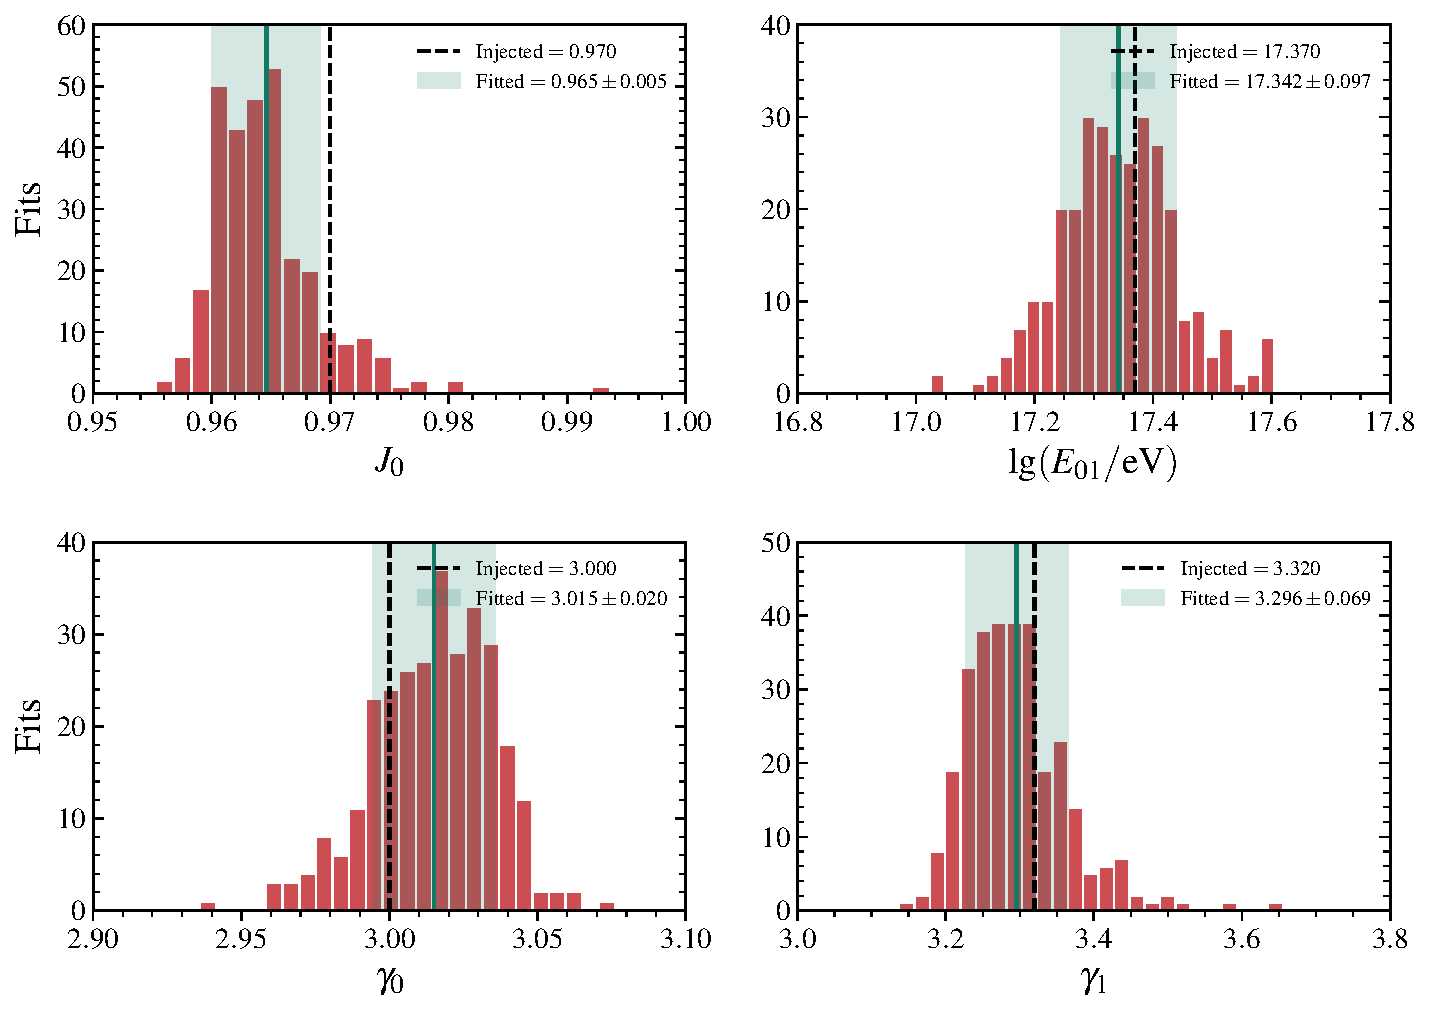
\includegraphics[width=\linewidth]{figures/chapter_spectrum/omega_wrong_closure_python.pdf}
    \caption{Distributions of the spectral parameters reconstructed from toy spectra generated with $\omega_{01}=0.25$ and fitted with a sharp transition fixed to $\omega_{01}=0.05$, as used for the measured data. The dashed vertical lines indicate the injected values, while the solid vertical lines show the mean fitted values and the shaded regions represent the corresponding $1\sigma$ intervals.}
    \label{fig:omega_wrong}
\end{figure}

To assess the effect of the assumed transition width on the other spectral parameters, the fit is repeated with $\omega_{01}$ fixed between $0$ and $0.5$ in steps of $0.05$, with $\omega_{01}=0$ corresponding to the sharp broken-power-law limit.
The resulting Poisson deviance, second-knee energy, and spectral indices are shown in \cref{fig:omega_study}.
The circles represent the fits with fixed $\omega_{01}$ and the stars indicate the result obtained when $\omega_{01}$ is left free.
%
The deviance varies by only approximately $1.6$ over the full scan, indicating that the \sd{433} data have little sensitivity to the transition width.
The reconstructed second-knee energy remains compatible within statistical uncertainties with the nominal result obtained for $\omega_{01}=0.05$.

A mild correlation is observed between the transition width and the spectral indices.
As $\omega_{01}$ increases, the fitted value of $\gamma_0$ decreases from approximately $3.04$ to $2.97$, while $\gamma_1$ increases from approximately $3.34$ to $3.38$.
This behavior reflects a compensation between the transition width and the asymptotic slopes: a broader transition is accommodated by a flatter spectrum below the second knee and a steeper spectrum above it.
Nevertheless, these variations remain compatible with the statistical uncertainties of the corresponding fits near the fitted $\omega_{01}$.

\begin{figure}
    \centering
    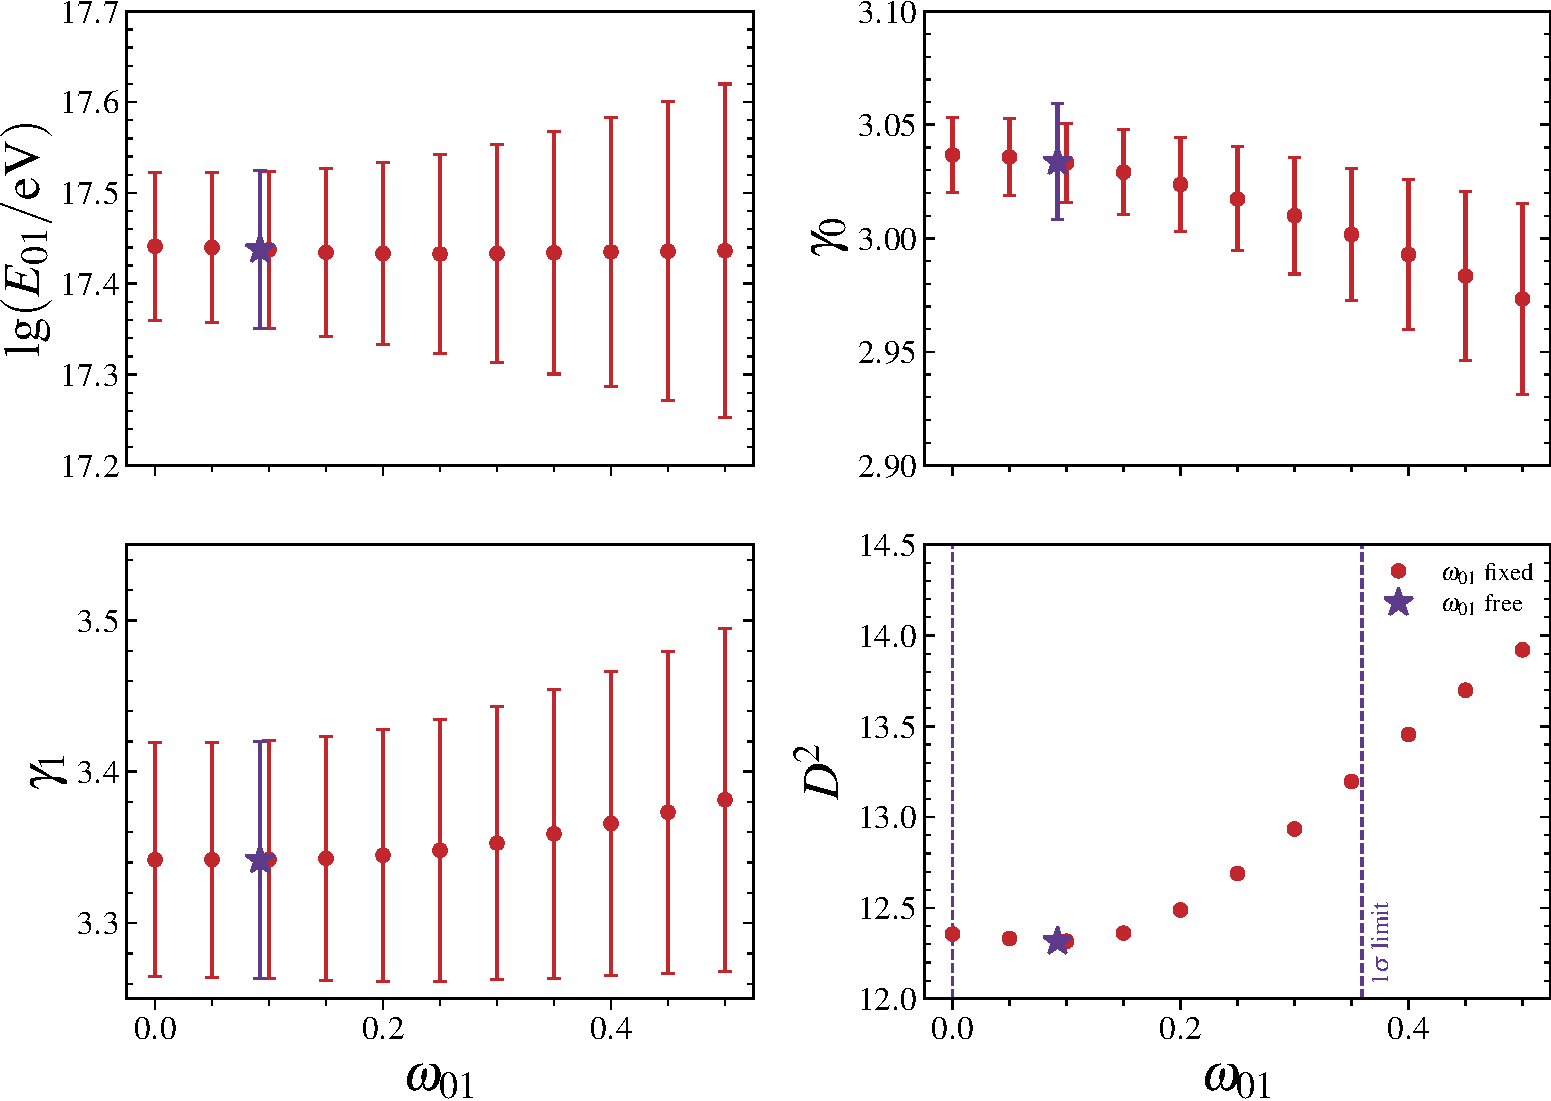
\includegraphics[width=\linewidth]{figures/chapter_spectrum/omega_dependence_2x2.pdf}
    \caption{
        Dependence of the fitted second-knee parameters and Poisson deviance
        on the assumed transition width $\omega_{01}$ for the \sd{433}
        spectrum. Circles show fits with $\omega_{01}$ fixed, while the star
        indicates the result obtained when $\omega_{01}$ is left free.
        The error bars represent the statistical uncertainties of the fits.
        The dashed vertical lines in the lower-right panel indicate the
        $1\sigma$ limits of the free-$\omega_{01}$ fit.
    }
    \label{fig:omega_study}
\end{figure}

The Monte Carlo studies and the scan of the transition width highlight that fixing $\omega_{01}=0.05$ in the fit does not introduce a significant bias in the reconstructed second-knee energy or spectral indices, even if the injected transition is substantially broader.
No additional systematic uncertainty is therefore assigned to the choice of $\omega_{01}$.

A summary of the contributions to the systematic uncertainties of the fitted spectral parameters is presented in \cref{table:sd433_parameter_systematics}.
The FD energy scale dominates the uncertainties in the normalization and second-knee energy, while the calibration parameters provide the largest contribution to the uncertainties in the spectral indices.
The detector-response uncertainties are subdominant throughout the measured energy range, and the exposure uncertainty affects only the normalization.
Since the different sources are treated as uncorrelated, the total systematic uncertainty for each parameter is obtained by adding the individual contributions in quadrature.

\begin{table}
    \centering
    \caption{Contributions to the systematic uncertainties of the fitted \sd{433} spectral parameters. The values correspond to the largest absolute variation obtained for each source. The uncertainty in $J_0$ is expressed in units of $10^{-13}\,\mathrm{km^{-2}\,yr^{-1}\,sr^{-1}\,eV^{-1}}$. The total is obtained by adding the independent contributions in quadrature.}
    \label{table:sd433_parameter_systematics}
    \begin{tabular}{lcccc}
        \hline
        Source
        & $\Delta J_0$
        & $\Delta\lg(E_{01}/\mathrm{eV})$
        & $\Delta\gamma_0$
        & $\Delta\gamma_1$ \\
        \hline
        FD energy scale
        & $0.277$ & $0.100$ & $0.024$ & $0.055$ \\
        Calibration
        & $0.156$ & $0.024$ & $0.083$ & $0.095$ \\
        Energy resolution
        & $0.008$ & $0.003$ & $0.005$ & $0.002$ \\
        Composition: bias
        & $0.038$ & $0.006$ & $0.026$ & $0.019$ \\
        Composition: efficiency
        & $0.005$ & $0.032$ & $0.019$ & $0.011$ \\
        Exposure
        & $0.028$ & $0$ & $0$ & $0$ \\
        \hline
        \textbf{Total}
        & $\mathbf{0.321}$
        & $\mathbf{0.108}$
        & $\mathbf{0.092}$
        & $\mathbf{0.112}$ \\
        \hline
    \end{tabular}
\end{table}

\begin{table}
    \centering
    \caption{
        Best-fit values of the \sd{433} spectral parameters.
        The first uncertainty is statistical and the second systematic.
        The transition width is fixed in the fit.
    }
    \label{table:sd433_spectral_parameters}
    \begin{tabular}{lc}
        \hline
        Parameter & Value $\,\pm\sigma_{\mathrm{stat}}\pm\sigma_{\mathrm{syst}}$ \\
        \hline
        $J_0/
        \left(
        \mathrm{km^{-2}\,yr^{-1}\,sr^{-1}\,eV^{-1}}
        \right)$
        & $(0.912\pm0.005\pm0.321)\times10^{-13}$ \\
        $\gamma_0$
        & $3.04\pm0.02\pm0.09$ \\
        $E_{01}/\mathrm{eV}$
        & $(2.8\pm0.5\pm0.7)\times10^{17}$ \\
        $\gamma_1$
        & $3.34\pm0.08\pm0.11$ \\
        $\omega_{01}$
        & $0.05$ (fixed) \\
        \hline
    \end{tabular}
\end{table}

\section{Summary of the chapter}

This chapter presents the measurement of the cosmic-ray energy spectrum with the \sd{433} array using data reconstructed in the previous chapter and recorded between July 2018 and December 2021.
The raw flux was obtained from the observed event counts and the geometrical exposure, as determined in \cref{chap:sd433_dataset}.

To correct for detector effects in the spectrum measurement, a forward-folding procedure was developed and included in the spectrum fit.
The detector response was incorporated into a migration matrix describing the probability that an event with true energy in bin $j$ is reconstructed in bin $i$.
The matrix accounts for the energy-dependent detection efficiency, bias, and finite resolution of the \sd{433}.
Although its exact definition depends on the assumed spectral model, this dependence can be neglected when the true-energy binning is sufficiently fine.
A true-energy bin width of $\Delta\lg(E_j/\mathrm{eV})=0.01$ was therefore adopted, compared with $\Delta\lg(E_i/\mathrm{eV})=0.1$ in reconstructed energy.

This approximation was benchmarked before being applied to the measured spectrum.
The expected reconstructed event counts obtained with the approximate matrix were compared with those calculated using the exact, spectrum-dependent expression for an injected power-law spectrum.
The relative differences were found to be negligible across the full energy range.
This validation showed that the approximate matrix preserves the detector response while avoiding the need to assume the spectral parameters a priori and to recalculate the matrix at every step of the fit.

The validated migration matrix was subsequently used in a Poisson-likelihood fit to predict the number of events in each bin.
Once the best-fit spectral parameters were obtained, the ratio between the expected true and reconstructed event counts provided the correction factors used to unfold the measured flux.

A simple power law model for the flux is rejected with a $p$-value of
\SDFourThreeThreePowerLawPValue, providing evidence for a change in the spectral slope.
The spectrum is therefore described using a broken power law with a smooth transition.
The complete set of fitted parameters is summarized in
\cref{table:sd433_spectral_parameters}.

The available \sd{433} statistics are insufficient to constrain the transition width; therefore, this parameter is fixed to $\omega_{01}=0.05$, following the value adopted by the Pierre Auger Observatory for spectral features whose transition widths could not be constrained.
Our analysis shows that this choice does not introduce a significant bias in the reconstructed second-knee energy or spectral indices.
The transition width will be investigated with greater sensitivity using the combined \sd{433} and \sd{750} spectrum, thanks to the larger statistics available in the latter.

The systematic study identifies the inherited \gls{fd} energy-scale uncertainty as the dominant contribution to the flux normalization and the position of the second knee.
The systematic uncertainty in the \sd{433} energy calibration parameters produces the next-largest contribution to the flux and has the strongest effect on the spectral indices, while uncertainties associated with the detector response lead to smaller contributions.
Overall, the measurement establishes the spectral increase in the energy range covered by \sd{433} and measures all related spectral parameters with their corresponding statistical and systematic uncertainties.

\end{document}
